\documentclass[aspectratio=169,professionalfonts]{beamer}

% --- Encoding & fonts (pdflatex-safe) ---------------------------------
\usepackage[T1]{fontenc}
\usepackage[utf8]{inputenc}
\usepackage[spanish, es-nodecimaldot]{babel}

\usepackage{amsmath}
\usepackage{amssymb}
\usepackage{amsthm}
\usepackage{mathtools}

\usepackage{lmodern}
\usepackage[protrusion=true,expansion=true,tracking=true]{microtype}
\usepackage{amsmath,amssymb,mathtools}
\usepackage[dvipsnames]{xcolor}

\usepackage{subcaption}
\usepackage{caption}

\usepackage{graphicx}
\usepackage{geometry}

\usepackage{tikz}
\usetikzlibrary{intersections}
\usetikzlibrary{babel}

\usepackage{pgfplots}
\pgfplotsset{compat=1.18}
\usepgfplotslibrary{fillbetween}

\usepackage{bookmark}

% --- Color palette (monochrome-forward) --------------------------------
\definecolor{Ink}{RGB}{20,20,20}       % near-black for text
\definecolor{Paper}{RGB}{255,255,255}  % white background
\definecolor{Rule}{gray}{0.65}         % hairline rules & leaders
\definecolor{Mute}{gray}{0.45}         % muted annotations

\setbeamercolor{normal text}{fg=Ink,bg=Paper}
\setbeamercolor{structure}{fg=Ink}
\setbeamercolor{frametitle}{fg=Ink,bg=Paper}
\setbeamercolor{title}{fg=Ink}
\setbeamercolor{subtitle}{fg=Mute}
\setbeamercolor{footline}{fg=Mute,bg=Paper}
\setbeamercolor{block title}{fg=Ink,bg=Paper}
\setbeamercolor{block body}{fg=Ink,bg=Paper}

% --- Typography ---------------------------------------------------------
\setbeamerfont{title}{series=\bfseries,size=\fontsize{22}{26}}
\setbeamerfont{subtitle}{series=\mdseries,size=\fontsize{12}{14}}
\setbeamerfont{frametitle}{series=\bfseries,size=\fontsize{18}{22}}
\setbeamerfont{normal text}{size=\fontsize{11}{13}}
\setbeamerfont{block title}{series=\bfseries}
% \SetTracking{encoding=*}{0} % base

% small caps with subtle letterspacing (book uses uppercase/small caps)
\newcommand{\PLcaps}[1]{{\addfontfeatures{}\textls[120]{\scshape #1}}}
\newcommand{\PLupper}[1]{\textls[5]{\MakeUppercase{#1}}}

% --- Remove navigation symbols ----------------------------------------
\setbeamertemplate{navigation symbols}{}

% --- Headline: none (clean pages, like the book) -----------------------
\setbeamertemplate{headline}{}

% --- Footline: thin rule + title left, frame numbers right --------------
\setbeamertemplate{footline}{%
  \begin{beamercolorbox}[wd=\paperwidth,ht=0.75ex,dp=0ex]{}
    \color{Rule}\rule{\paperwidth}{0.4pt}% hairline
  \end{beamercolorbox}%
  \vspace{0.25ex}%
  \begin{beamercolorbox}[wd=\paperwidth,ht=2.8ex,dp=1.0ex,left]{footline}
    \hspace*{0.8ex}\usebeamerfont{footline}\textls[80]{\insertshorttitle}
    \hfill\insertframenumber{} / \inserttotalframenumber\hspace*{0.8ex}
  \end{beamercolorbox}%
}

% --- Frametitle: uppercase + hairline underline ------------------------
\makeatletter
\setbeamertemplate{frametitle}{%
  {\usebeamerfont{frametitle}\PLupper{\insertframetitle}}\par
  \vspace{0.35ex}
  {\color{Rule}\rule{\linewidth}{0.6pt}}%
}
\makeatother

% --- Blocks: outlined (no fills), small caps titles ---------------------
\setbeamertemplate{blocks}[default]
\setbeamertemplate{block begin}{%
  {\usebeamerfont{block title}\insertblocktitle}
  {\color{Rule}\rule{\linewidth}{0.6pt}}
  \par\vspace{0.6ex}%
}
\setbeamertemplate{block end}{%
  {\color{Rule}\rule{\linewidth}{0.6pt}}% thin rule under title
  \par\vspace{0.6ex}
}
\setbeamertemplate{block alerted begin}{\setbeamercolor{block title}{fg=Ink}\setbeamercolor{block body}{fg=Ink}\usebeamertemplate{block begin}}
\setbeamertemplate{block alerted end}{\usebeamertemplate{block end}}
\setbeamertemplate{block example begin}{\usebeamertemplate{block begin}}
\setbeamertemplate{block example end}{\usebeamertemplate{block end}}

% --- Itemize: minimalist points & dashes -------------------------------
\setbeamertemplate{itemize item}{\raise0.2ex\hbox{\small\textbullet}}
\setbeamertemplate{itemize subitem}{\raise0.2ex\hbox{\scriptsize\textendash}}
\setbeamertemplate{itemize subsubitem}{\raise0.2ex\hbox{\tiny\textbullet}}
\setlength{\leftmargini}{1.5em}

% --- Table of contents with dotted leaders (no page numbers) -----------
% Custom section/subsection in toc templates using typographic leaders.
\def\PLleaders{\leaders\hbox{\color{Rule}.\kern0.3em}\hfill}

\defbeamertemplate{section in toc}{puntolinea}{%
  \par\vspace{0.4ex}%
  {\PLcaps{\inserttocsection}} \PLleaders{}\par
}
\defbeamertemplate{subsection in toc}{puntolinea}{%
  \hspace*{1.0em}{\footnotesize\inserttocsubsection} \PLleaders{}\par
}
\setbeamertemplate{section in toc}[puntolinea]
\setbeamertemplate{subsection in toc}[puntolinea]

% --- Title page (typographic, no graphics) -----------------------------
\defbeamertemplate*{title page}{puntolinea}{%
  \vspace*{10mm}% generous top margin
  {\usebeamerfont{title}\PLupper{\inserttitle}}\par
  \vspace{0.8ex}
  {\color{Rule}\rule{0.82\linewidth}{0.8pt}}\par
  \vspace{0.6ex}
  {\usebeamerfont{subtitle}\PLcaps{\insertsubtitle}}\par
  \vfill
  {\PLcaps{\insertauthor}}\par
  {\PLcaps{\insertinstitute}}\par
  {\PLcaps{\insertdate}}\par
}
\setbeamertemplate{title page}[puntolinea]

% --- Optional: section pages (uppercase heading with rule) -------------
\setbeamertemplate{section page}{%
  \vspace*{18mm}
  {\usebeamerfont{frametitle}\PLupper{\thesection.\ \insertsection}}\par
  \vspace{0.6ex}
  {\color{Rule}\rule{\linewidth}{0.8pt}}\par
}
\AtBeginSection{\begin{frame}[plain]\sectionpage\end{frame}}

% custom commands
\newcommand{\Z}{\mathbb{Z}}
\newcommand{\N}{\mathbb{N}}
\newcommand{\Q}{\mathbb{Q}}
\newcommand{\R}{\mathbb{R}}
\newcommand{\F}{\mathbb{F}}
\newcommand{\NIL}{\textnormal{\textsc{NIL}}}

% vectors and linear algebra
\newcommand{\norm}[1]{\left\lVert #1 \right\rVert}
\renewcommand{\ker}[1]{\mathop{\mathrm{ker}{\left\lbrace #1 \right\rbrace}}}
\renewcommand{\vec}[1]{\boldsymbol{#1}}
\newcommand{\inv}[1]{#1^{-1}}
\DeclarePairedDelimiter\braket{\langle}{\rangle}

% algebra
\DeclareMathOperator{\GL}{GL}
\newcommand{\glz}[2]{\GL_{#1}\left(#2\right)}
\DeclareMathOperator{\orb}{orb}
\newcommand{\uvec}[1]{\hat{\vec{#1}}}

% optimization
\DeclareMathOperator{\argmax}{arg\,max}

% convex geom
\DeclareMathOperator{\gen}{gen}
\DeclareMathOperator{\aff}{aff}
\DeclareMathOperator{\conv}{conv}

% shortcuts
\newcommand{\est}[1]{\hat{\vec{ #1 }}}
\newcommand{\optilp}[1]{#1^*_{\text{PE}}}
\newcommand{\optr}[1]{#1^*_{\text{PR}}}
\newcommand{\braces}[1]{\lbrace #1 \rbrace}
\newcommand{\paren}[1]{\left( #1 \right)}
\newcommand{\tvec}[1]{\vec{\tilde{#1}}}
\newcommand{\proy}[1]{\pi^{(#1)}}

\newcommand{\clayer}[2]{H_{#1, #2}}
\newcommand{\qlayer}[2]{\clayer{\vec{#1}}{#2\norm{\vec{#1}}^{-2}}}

\newcommand{\floor}[1]{\left\lfloor #1 \right\rfloor}
\newcommand{\ceil}[1]{\left\lceil #1 \right\rceil}

\renewcommand{\gcd}[1]{\mathop{\mathrm{mcd}{\left\lbrace #1 \right\rbrace}}}
\newcommand{\lcm}[1]{\mathop{\mathrm{mcm}{\left\lbrace #1 \right\rbrace}}}

\title[Punto y línea sobre el plano]{Punto y línea sobre el plano}
\subtitle{Ecuaciones lineales diofantinas aplicadas a programas lineales enteros}
\author[Iñaki Liendo]{Iñaki Liendo}
\institute[ITAM]{Coloquio de matemáticas}
\date{\today}

\begin{document}
\begin{frame}[plain]
	\titlepage
\end{frame}

% motivation
\section{Motivación}
\begin{frame}
	\begin{block}{Definición}
		Sea $\vec{a} \in \R^n$ un vector no nulo y sea $b \in \R$ un escalar. Llamamos
		\textbf{hiperplano afino} al conjunto de vectores $\vec{x} \in \R^n$ que satisfacen
		$\vec{a}^T\vec{x} = b$. Llamamos \textbf{semi-espacios afinos} a los conjuntos de vectores
		$\vec{x}, \vec{y} \in \R^n$ que satisfacen $\vec{a}^T\vec{x} \geq b$ y $\vec{a}^T\vec{y}
		\leq b$.
	\end{block}
\end{frame}

\begin{frame}
	\begin{block}{Definición}
		Sea $A \in \R^{m \times n}$ una matriz con renglones linealmente independientes y sea
		$\vec{b} \in \R^m$ un vector. Llamamos \textbf{poliedro} al conjunto definido por
		\begin{equation*}
			P \coloneq \braces{\vec{x} \in \R^n \vcentcolon A\vec{x} \leq \vec{b}}
			= \braces{\vec{x} \in \R^n \vcentcolon \vec{a}^T_i\vec{x} \leq b_i, 1 \leq i \leq m}.
		\end{equation*}
	\end{block}
\end{frame}

\begin{frame}
	\begin{figure}[ht]
		\centering
		\begin{minipage}{0.45\textwidth}
			\centering
			\begin{tikzpicture}[scale=1.1]
				% hyperplane
				\draw[ultra thick, black] (-2,1) -- (2,-2) node[above right] {$\vec{a}^T\vec{x} = b$};
				% labels
				\node at (-1.2,-1.2) {${\vec{a}^T \vec{x} \leq b}$};
				%shading
				\fill[Periwinkle!20, domain=-2:2, variable=\x]
					(-2,1) -- plot ({\x}, {-0.75*\x - 0.5}) -- (2,1) -- cycle;
				\draw[->, thick] (1,-1.25) -- (1.5,-0.583) node[right] {$\vec{a}$};
				\node at (0.8,0.5) {${\vec{a}^T \vec{x} \geq b}$};
			\end{tikzpicture}
		\end{minipage}
		\begin{minipage}{0.45\textwidth}
			\centering
			\begin{tikzpicture}[scale=2.0, >=stealth]
				% coordinates
				\coordinate (A) at (0,0);
				\coordinate (B) at (1.5,0);
				\coordinate (C) at (1.8,1);
				\coordinate (D) at (0.75,1.7);
				\coordinate (E) at (-0.3,1);
				% pentagon
				\filldraw[fill=Periwinkle!20, thick]
				(A) -- (B) -- (C) -- (D) -- (E) -- cycle;
			  % normal vectors
				% AB
				\draw[->, black, thick] (0.75,0) -- (0.75,0.46) node[below right] {$\vec{a}_1$};
				% BC
				\draw[->, black, thick] (1.65,0.5) -- (1.34,0.59) node[above right] {$\vec{a}_2$};
				% CD
				\draw[->, black, thick] (1.275,1.35) -- (1.06,1.027) node[above left] {$\vec{a}_3$};
				% DE
				\draw[->, black, thick] (0.225,1.35) -- (0.44,1.027) node[below left] {$\vec{a}_4$};
				% EA
				\draw[->, black, thick] (-0.15,0.5) -- (0.157,0.592) node[below right] {$\vec{a}_5$};
				% polyhedron label
				\node at (0.75, 0.75) {$P$};
			\end{tikzpicture}
		\end{minipage}
	\end{figure}
\end{frame}

\begin{frame}
	\begin{block}{Definición}
		Sea $P \subseteq \R^m$ un poliedro y sea $\vec{c} \in \R^n$ un vector. Llamamos
		\textbf{problema lineal} al problema de maximización
		\begin{equation*}
			z^* \coloneq \max_{\vec{x}}\braces{\vec{c}^T\vec{x} \vcentcolon \vec{x} \in P}.
		\end{equation*}
	\end{block}
	\textbf{Nota:} Un problema lineal puede ser infactible porque $P$ es vacío (y entonces $z^*$ no
	está bien definida) o puede ser no acotado porque $z^* = \infty$.
\end{frame}

\begin{frame}
	\begin{block}{Teorema}
		Supongamos que el valor óptimo $z^*$ existe y es finito. Entonces el conjunto de soluciones
		óptimas $\braces{\vec{x}^* \in P \vcentcolon \vec{c}^T\vec{x}^* = z^*}$ contiene al menos un
		vértice de $P$.
	\end{block}
\end{frame}

\begin{frame}
	\begin{figure}[ht]
		\centering
		\begin{tikzpicture}[scale=2.0, >=stealth]
			% coordinates
			\coordinate (A) at (0,0);
			\coordinate (B) at (1.5,0);
			\coordinate (C) at (1.8,1);
			\coordinate (D) at (0.75,1.7);
			\coordinate (E) at (-0.3,1);
			% pentagon
			\filldraw[fill=Periwinkle!20, thick]
			(A) -- (B) -- (C) -- (D) -- (E) -- cycle;
			\draw[->, black, thick] (0,0) -- (0.4, 0.6) node[below right] {$\vec{c}$};
		\end{tikzpicture}
	\end{figure}
\end{frame}

\begin{frame}
	\begin{figure}[ht]
		\centering
		\begin{tikzpicture}[scale=2.0, >=stealth]
			% coordinates
			\coordinate (A) at (0,0);
			\coordinate (B) at (1.5,0);
			\coordinate (C) at (1.8,1);
			\coordinate (D) at (0.75,1.7);
			\coordinate (E) at (-0.3,1);
			% pentagon
			\filldraw[fill=Periwinkle!20, thick]
			(A) -- (B) -- (C) -- (D) -- (E) -- cycle;
			\draw[dash pattern={on 7pt off 2pt on 1pt off 3pt}, black, thick] (0,0) -- (1.015, 1.523);
			\draw[->, black, thick] (0,0) -- (0.4, 0.6) node[below right] {$\vec{c}$};
			\draw[black] (1.015,1.523) -- (0.954,1.431) -- (1.059,1.361) -- (1.120,1.453);
			\draw[black, ultra thick] (C) -- (D);
		\end{tikzpicture}
	\end{figure}
\end{frame}

\begin{frame}
	\begin{block}{Definición}
		Al problema lineal
		\begin{equation*}
			z^* \coloneq \max_{\vec{x}}\braces{\vec{c}^T\vec{x} \vcentcolon \vec{x} \in P}.
		\end{equation*}
		lo llamamos \textbf{problema relajado} del \textbf{problema lineal entero}
		\begin{equation*}
			\optilp{z} \coloneq \max_{\vec{x}}\braces{\vec{c}^T\vec{x} \vcentcolon \vec{x} \in P \cap \Z^n}.
		\end{equation*}
	\end{block}
	\textbf{Nota:} Como $P \cap \Z^n \subseteq P$, tenemos $\optilp{z} \leq z^*$.
\end{frame}

\begin{frame}
	\begin{figure}
		\centering
		\begin{tikzpicture}[scale=1]
			\begin{axis}[
				axis lines=left,
				xmin=-0.5, xmax=3.5,
				ymin=-0.5, ymax=3.5,
				grid=both,
				xlabel=$x_1$,
				ylabel=$x_2$
				]
				\addplot+ [
				  thick, color=black, fill=WildStrawberry!20, mark=none
				] coordinates {
				  (0,0)
				  (1.5,0)
				  (2.2,0.7)
				  (2.8,3)
				  (0,3)
				  (0,0)
				};
				\addplot+[
				  only marks, mark=*,
				  mark options={scale=1.1, color=black, fill=Goldenrod!50}
				] coordinates {
				  (0,0) (0,1) (0,2) (0,3)
				  (1,0) (1,1) (1,2) (1,3)
				  (2,1) (2,2) (2,3)
				};
				\draw[->, thick, color=ForestGreen] (axis cs:0,3) -- (axis cs:1,2.75);
			\end{axis}
		\end{tikzpicture}
	\end{figure}
\end{frame}

\begin{frame}
	\begin{figure}
		\centering
		\begin{tikzpicture}[scale=0.7]
			\begin{axis}[
			  axis lines=middle,
			  xmin=0, xmax=1.2,
			  ymin=0, ymax=1.2,
			  xlabel={$x$}, ylabel={$y$},
			  clip=false
			]
				\addplot [name path=top, draw=none, domain=0:1.2] {1.2};
				\addplot [name path=lower, draw=none, samples=200, domain=0:1.2]
				  {max(x-0.3, 0)};
				\addplot [Plum!25] fill between[of=top and lower];
				\addplot [black, thick, domain=0.3:1.2] {x - 0.3};
				\addplot [black, thick, domain=0:0.3] {0};
				\node at (axis cs:0.5,0.7) {\Large $S_{0}$};
				\draw[->, thick, black] (0.6, 0.3) -- (0.8, 0.1);
				\draw[black] (0.6,0.3) -- (0.579,0.279) -- (0.599,0.259) -- (0.62,0.28);
			\end{axis}
		\end{tikzpicture}
	\end{figure}
\end{frame}

\begin{frame}
	\begin{figure}
		\centering
		\begin{tikzpicture}[scale=0.7, >= stealth]
			\begin{axis}[
			  axis lines=middle,
			  xmin=1, xmax=2.2,
			  ymin=1, ymax=2.2,
			  xlabel={$x$}, ylabel={$y$},
			  clip=false
			]
				\addplot [name path=top, draw=none, domain=1:2.2] {2.2};
				\addplot [name path=lower, draw=none, samples=200, domain=1:2.2]
				  {1 + max(x-1.3, 0)};
				\addplot [Plum!25] fill between[of=top and lower];
				\addplot [black, thick, domain=1.3:2.2] {x - 0.3};
				\addplot [black, thick, domain=1:1.3] {1};
				\node at (axis cs:1.5,1.7) {\Large $S_{011}$};
				\draw[->, thick, black] (1.6, 1.3) -- (1.8, 1.1);
				\draw[black] (1.6,1.3) -- (1.579,1.279) -- (1.599,1.259) -- (1.62,1.28);
			\end{axis}
		\end{tikzpicture}
	\end{figure}
\end{frame}

\begin{frame}
	Ramificación y Acotamiento genera la cadena de subproblemas autosimilares
	\begin{equation*}
		S_{0}, S_{011}, S_{01111}, S_{0111111}, \ldots,
	\end{equation*}
	y este método jamás terminará con una solución.
\end{frame}

\begin{frame}
	En general, Ramificación y Acotamiento es ineficiente (o incluso falla) cuando una
	restricción del problema es ortogonal al vector objetivo. La instancia minimal que reproduce
	esta ineficiencia es
	\begin{subequations}
		\label{theory:formulation}
		\begin{align}
			\max_{\vec{x} \in \Z^n} \quad
				& \vec{p}^T\vec{x}, \label{theory:objective} \\
			\text{s.a.} \quad
				& \vec{p}^T\vec{x} \leq u, \label{theory:constraint:budget} \\
				& \vec{x} \geq \vec{0}. \nonumber
		\end{align}
	\end{subequations}
\end{frame}

\begin{frame}
	Aún más general, Ramificación y Acotamiento es ineficiente cuando el
	problema contiene múltiples simetrías:
	\begin{figure}
		\includegraphics[width=0.4\linewidth]{/home/tempdata/Pictures/chesslp.jpeg}
	\end{figure}
\end{frame}

\begin{frame}
	\begin{itemize}
		\item Sin contar rotaciones o reflexiones del tablero, cada solución
			tiene al menos
		\begin{equation*}
			8! \times (2!)^3 \times 1! \times 1! = 322{,}560
		\end{equation*}
		soluciones equivalentes.
		\item Contanto rotaciones y reflexiones del tablero, cada solución
			tiene al menos
		\begin{equation*}
			4 \times 2 \times 322{,}560 = 2{,}580{,}480
		\end{equation*}
		soluciones equivalentes.
		\item Las simetrías dependen de la formulación que utilicemos. Si la
			formulación induce a que las soluciones equivalentes se encuentren
			en árboles disjuntos, entonces estos jamás serán podados y
			Ramificación y Acotamiento es más ineficiente.
		\item ¿Cuántas soluciones distintas (no equivalentes) existen?
	\end{itemize}
\end{frame}

% \begin{frame}
% 	\begin{figure}
% 		\centering
% 		\begin{tikzpicture}[scale=1, node/.style={draw, thick}]
% 			\node[node] (Start) at (0,6) {Inicio};
% 			\node[node] (Presolve) at (3,6) {Presolución};
% 			\node[node] (Return) at (6,5) {Devolver};
% 			\node[node] (Node selection) at (3,5) {Selección de nodos};
% 			\node[node] (LP relaxation) at (3,4) {Problema relajado};
% 			\node[node] (Cuts) at (3,3) {Cortes};
% 			\node[node] (Branching) at (3,2) {Ramificación};
% 			\node[node] (Heuristics) at (6,3) {Heurísticas};
% 			% Arrows
% 			\draw[thick, ->] (Start) --(Presolve);
% 			\draw[thick, ->] (Presolve) -- (Node selection);
% 			\draw[thick, ->] (Presolve) -- (6,6) -- (Return);
% 			\draw[thick, ->] (Node selection) -- (LP relaxation);
% 			\draw[thick, ->] (Node selection) -- (Return);
% 			\draw[thick, ->] (LP relaxation) -- (Cuts);
% 			\draw[thick, ->] (LP relaxation) -- (6,4) -- (Heuristics);
% 			\draw[thick, ->] (Cuts) -- (Branching);
% 			\draw[thick, ->] (Heuristics) -- (Cuts);
% 			\draw[thick, ->] (Branching) -- (0,2) -- (0,5) --(Node selection);
% 			\draw[thick, ->] (Cuts) -- (0.5,3) -- (0.5,4) -- (LP relaxation);
% 		\end{tikzpicture} 
% 	\end{figure}
% \end{frame}

% \begin{frame}
% 	\begin{figure}[hbtp]
% 	  \centering
% 	  \begin{subfigure}{0.45\textwidth}
% 		\centering
% 		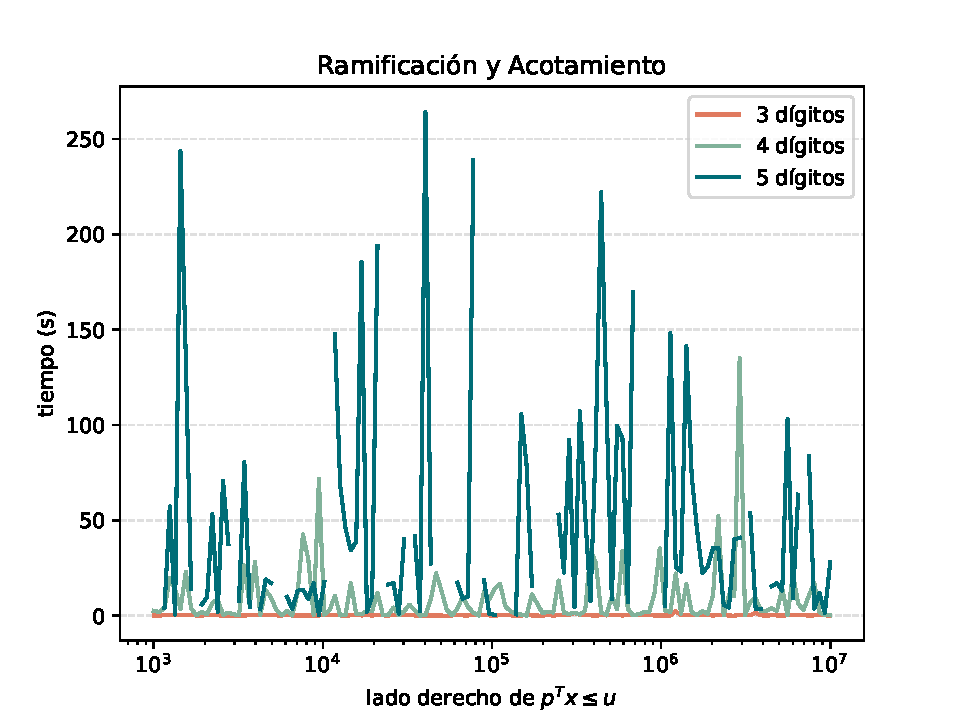
\includegraphics[width=\linewidth]{/home/tempdata/repos/thesis/static/inf/digits-bb_full.pdf}
% 	  \end{subfigure}
% 	  \hfill
% 	  \begin{subfigure}{0.45\textwidth}
% 		\centering
% 		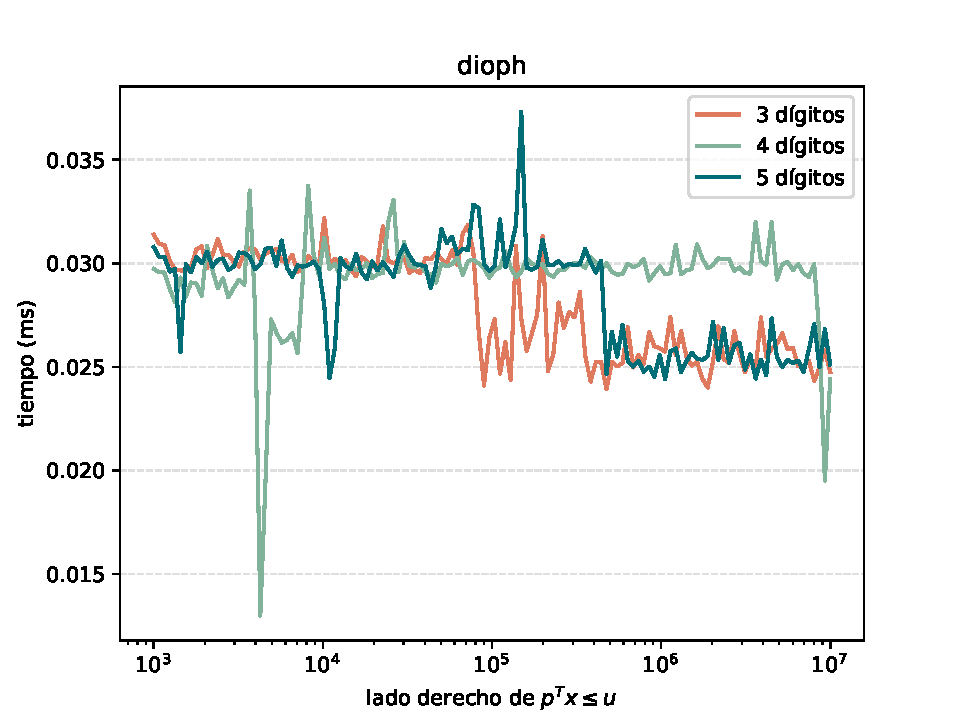
\includegraphics[width=\linewidth]{/home/tempdata/repos/thesis/static/inf/digits-dioph.pdf}
% 	  \end{subfigure}
%   \end{figure}
% \end{frame}


% c-layers
\section{Fundamentos}

\subsection{Capas enteras}
\begin{frame}
	\begin{block}{Definición}
		Decimos que un vector $\vec{v} \in \R^n \setminus \braces{\vec{0}}$ es
		\textbf{esencialmente entero} si existen un vector $\vec{w} \in \Z^n$ y
		un escalar $m \neq 0$ tales que $\vec{v} = m\vec{w}$. Además, decimos
		que $\vec{w}$ es el \textbf{múltiplo coprimo} de $\vec{v}$ si sus
		entradas son coprimas y si su primera entrada no nula es positiva.
	\end{block}
\end{frame}

\begin{frame}
	\begin{block}{Ejemplo}
		El vector $(-\sqrt{2}, 1/\sqrt{2}) = 2\sqrt{2}(-2, 1)$ es
		esencialmente entero y $(2, -1)$ es su múltiplo coprimo. En contraste,
		el vector $\paren{\sqrt{2}, \sqrt{3}}$ no es esencialmente entero (¿por
		qué?).
	\end{block}
	\begin{itemize}
		\item \textbf{Ejercicio:} Todo vector racional $\vec{v} \in \Q^n$ no
			nulo es esencialmente entero.
		\item $\implies$ Todo número representable en un sistema de aritmética
			finita es esencialmente entero.
	\end{itemize}
\end{frame}

\begin{frame}
	\begin{block}{Definición}
		Sea $\vec{v} \in \R^n$ un vector esencialmente entero y sea $t \in \R$ un
		escalar. Decimos que su hiperplano afino asociado
		\begin{equation*}
			\clayer{\vec{v}}{t} \coloneq \ker{\vec{x} \mapsto \vec{v}^T\vec{x}} + t\vec{v}
			= \lbrace \vec{v}^{\perp} + t\vec{v} \vcentcolon \vec{v}^T\vec{v}^{\perp} = 0 \rbrace
		\end{equation*}
		es una \textbf{capa entera} si contiene al menos un punto entero.
	\end{block}
	\begin{block}{Teorema de cobertura}
		Sea $\vec{v} \in \R^n$ un vector esencialmente entero y sea $\vec{w}$ su
		múltiplo coprimo. Entonces la familia de capas enteras
		$\braces{\qlayer{w}{k} \vcentcolon k \in \Z}$ cubre a
		$\Z^n$.
	\end{block}
\end{frame}

\begin{frame}
	\begin{block}{Lema de utilidad (*)}
		Sea $\vec{v} \in \R^n$ un vector esencialmente entero y sea $\vec{w}$ su
		múltiplo coprimo. Entonces $\vec{w}^T\vec{x} = k$ para todo $\vec{x} \in
		\qlayer{w}{k}$.
	\end{block}
	\begin{block}{Lema de satisfacción (*)}
		Sea $\vec{p} \in \R^n$ un vector esencialmente entero y sea $\vec{q}$ su
		múltiplo coprimo, de manera que $\vec{p} = m\vec{q}$ para algún escalar $m
		\neq 0$. Entonces la primera capa entera $\qlayer{q}{\eta}$ que satisface
		la restricción $\vec{p}^T\vec{x} \leq u$ está parametrizada por
		\begin{equation*}
			\label{lemma:eq:eta-cases}
			\eta \coloneq \begin{cases}
				\ceil{u/m}, & m < 0, \\
				\floor{u/m}, & m > 0.
			\end{cases}
		\end{equation*}
	\end{block}
\end{frame}

\begin{frame}
	\begin{block}{Teorema de infactibilidad (*)}
		Sea $\vec{p} \in \R^n$ un vector esencialmente entero y sea $\vec{q}$ su
		múltiplo coprimo. Entonces el problema \eqref{theory:formulation} es
		infactible si y solo si $\vec{q} \geq \vec{0}$ y el lado derecho $u$ de
		\eqref{theory:constraint:budget} es negativo. 
	\end{block}
\end{frame}

\begin{frame}
	\begin{block}{Teorema de factibilidad}
	Sea $\vec{p} \in \R^n$ un vector esencialmente entero y sea $\vec{q}$ su
	múltiplo coprimo, de manera que $\vec{p} = m\vec{q}$ para alguna $m > 0$.
	Supongamos que el problema \eqref{theory:formulation} es factible. Entonces
	se satisface lo siguiente:
	\begin{enumerate}
		\item Si $q_i < 0$ para algún $i \in \braces{1, \ldots, n}$, entonces la
			$\eta$-ésima capa entera $\qlayer{q}{\eta}$ contiene un número
			infinito de puntos factibles.
		\item Si $\vec{q} > \vec{0}$ entonces, para todo $k \in \braces{\eta,
			\eta - 1, \ldots, 0}$, la $k$-ésima capa entera $\qlayer{q}{k}$
			contiene un número finito de puntos factibles.
	\end{enumerate}
	\end{block}
\end{frame}

\begin{frame}
	\centering
	\begin{figure}
		\begin{tikzpicture}[scale=0.7]
			\begin{axis}[
			  axis lines=middle,
			  xmin=0, xmax=3.2,
			  ymin=0, ymax=3.2,
			  xlabel={$x$}, ylabel={$y$},
			  clip=false
			]
				\addplot [name path=top, draw=none, domain=0:3.2] {3.2};
				\addplot [name path=lower, draw=none, samples=200, domain=0:3.2]
				  {max(x-0.3, 0)};
				\addplot [OrangeRed!25] fill between[of=top and lower];
				\addplot [dash pattern={on 7pt off 2pt on 1pt off 3pt}, black, thick, domain=0.0:3.2] {x};
				\addplot [
				  only marks, mark=*,
				  mark options={scale=1.3, color=black, fill=Magenta!50}
				] coordinates {
				  (0,0)
				  (0,1)
				  (0,2)
				  (0,3)
				  (1,1)
				  (1,2)
				  (1,3)
				  (2,2)
				  (2,3)
				  (3,3)
				};
			\end{axis}
		\end{tikzpicture}
		\caption*{$x - y \leq 3.2$}
	\end{figure}
\end{frame}

\begin{frame}
	\centering
	\begin{minipage}{0.45\textwidth}
		\begin{figure}
			\begin{tikzpicture}[scale=0.7]
				\begin{axis}[
				  axis lines=middle,
				  xmin=0, xmax=3.3,
				  ymin=0, ymax=3.3,
				  xlabel={$x$}, ylabel={$y$},
				  clip=false
				]
					\addplot [name path=top, draw=none, domain=0:3.2] {0.0};
					\addplot [name path=lower, draw=none, samples=200, domain=0:3.2]
						{3.2 - x};
					\addplot [OrangeRed!25] fill between[of=top and lower];
					\addplot [dash pattern={on 7pt off 2pt on 1pt off 3pt}, black,
						thick, domain=0.0:3.0] {3 - x};
					\addplot [dash pattern={on 7pt off 2pt on 1pt off 3pt}, black,
						thick, domain=0.0:2.0] {2 - x};
					\addplot [dash pattern={on 7pt off 2pt on 1pt off 3pt}, black,
						thick, domain=0.0:1.0] {1 - x};
					\addplot [
					  only marks, mark=*,
					  mark options={scale=1.3, color=black, fill=Magenta!50}
					] coordinates {
					  (0,0)
					  (0,1)
					  (0,2)
					  (0,3)
					  (1,0)
					  (1,1)
					  (1,2)
					  (2,0)
					  (2,1)
					  (3,0)
					};
				\end{axis}
			\end{tikzpicture}
			\caption*{$x + y \leq 3.2$}
		\end{figure}
	\end{minipage}
	\begin{minipage}{0.45\textwidth}
		\begin{figure}
			\begin{tikzpicture}[scale=0.7]
				\begin{axis}[
				  axis lines=middle,
				  xmin=0, xmax=3.3,
				  ymin=0, ymax=3.3,
				  xlabel={$x$}, ylabel={$y$},
				  clip=false
				]
					\addplot [name path=top, draw=none, domain=0:3.2] {0.0};
					\addplot [name path=lower, draw=none, samples=200, domain=0:2.909090909]
						{(3.2 - 1.1*x)/1.3};
					\addplot [OrangeRed!25] fill between[of=top and lower];
					\addplot [black, domain=0.0:2.909090909] {(3.2 - 1.1*x)/1.3};
					\addplot [black, domain=0.0:2.818181818] {(3.1 - 1.1*x)/1.3};
					\addplot [black, domain=0.0:2.727272727] {(3.0 - 1.1*x)/1.3};
					\addplot [black, domain=0.0:2.636363636] {(2.9 - 1.1*x)/1.3};
					\addplot [black, domain=0.0:2.545454545] {(2.8 - 1.1*x)/1.3};
					\addplot [black, domain=0.0:2.454545455] {(2.7 - 1.1*x)/1.3};
					\addplot [thick, dash pattern={on 7pt off 2pt on 1pt off
						3pt}, black, domain=0.0:2.363636364] {(2.6 - 1.1*x)/1.3};
					\addplot [black, domain=0.0:2.272727273] {(2.5 - 1.1*x)/1.3};
					\addplot [dash pattern={on 7pt off 2pt on 1pt off 3pt}, black,
						thick, domain=0.0:2.18181818] {(2.4 - 1.1*x)/1.3};
					\addplot [black, domain=0.0:2.090909091] {(2.3 - 1.1*x)/1.3};
					\addplot [dash pattern={on 7pt off 2pt on 1pt off 3pt}, black,
						thick, domain=0.0:2] {(2.2 - 1.1*x)/1.3};
					\addplot [
					  only marks, mark=*,
					  mark options={scale=1.3, color=black, fill=Magenta!50}
					] coordinates {
						(0, 0)
						(1, 1)
						(0, 2)
						(2, 0)
					};
				\end{axis}
			\end{tikzpicture}
			\caption*{$1.1x + 1.3y \leq 3.2$}
		\end{figure}
	\end{minipage}
\end{frame}

\begin{frame}
	Por el teorema de factibilidad (o el de cobertura), las soluciones se
	encuentran en una capa entera $\qlayer{q}{k}$ con $0 \leq k \leq \eta$. Por
	el lema de utilidad, estas soluciones satisfacen la \textbf{ecuación lineal
	diofantina}
	\begin{equation*}
		\vec{q}^T\vec{x} = q_1x_1 + \cdots + q_nx_n = k.
	\end{equation*}
	Podemos resolver recursivamente esta ecuación. Utilizando una formulación
	hacia adelante, obtenemos...
\end{frame}

% \begin{frame}
% 	\begin{block}{Teorema de construcción}
% 		Sea $(x_0, y_0)$ una solución particular de la ecuación lineal
% 		diofantina $ax + by = c$. Entonces \textbf{todas} las soluciones enteras
% 		de aquella ecuación están dadas por
% 		\begin{equation}
% 			\label{prerreq:eq:construction}
% 			\begin{cases}
% 				x = x_0 + \frac{b}{d}t, \\
% 				y = y_0 - \frac{a}{d}t,
% 			\end{cases}
% 		\end{equation}
% 		donde $d \coloneq \gcd{a, b}$ y $t \in \Z$ es una variable libre.
% 	\end{block}
% \end{frame}
% 
% \begin{frame}
% 	\begin{block}{Teorema de existencia}
% 		Sean $a$ y $b$ enteros, no ambos iguales a cero. Entonces la ecuación lineal
% 		diofantina $ax + by = c$ tiene solución entera si y solo si $\gcd{a, b} \mid
% 		c$.
% 	\end{block}
% 	\begin{block}{Definición}
% 		Sea $d \coloneq \gcd{a, b}$ y sean $x', y'$ enteros tales que $ax' + by'
% 		= d$. Decimos entonces que $x', y'$ son \textbf{coeficientes de Bézout}
% 		asociados a $a$ y $b$, respectivamente
% 	\end{block}
% \end{frame}
% 
% \begin{frame}
% 	Definamos $d \coloneq \gcd{a, b}$ y supongamos que la ecuación $ax + by = c$
% 	tiene solución. Por el teorema de existencia se sigue que $d
% 	\mid c$, y entonces existe $c' \in \Z$ tal que $c = c' \cdot d$. Sean $x',
% 	y'$ los coeficientes de Bézout asociados a $a, b$ respectivamente. Así,
% 	\begin{equation*}
% 		a(c' \cdot x') + b(c' \cdot y') = c'(ax' + by') = c'd = c,
% 	\end{equation*}
% 	por lo que $(c' \cdot x', c' \cdot y')$ es una solución particular de la
% 	ecuación $ax + by = c$.
% \end{frame}
% 
% \begin{frame}
% 	Nuestro vector $\vec{q} = (q_1, q_2) \in \Z^2$ es coprimo. Es decir,
% 	$\gcd{q_1, q_2} = 1$. Luego, una solución particular de la ecuación lineal
% 	diofantina $q_1x_1 +q_2x_2 = k$ es $(x_1, x_2) = (kx_1', kx_2')$. En efecto,
% 	\begin{equation*}
% 		q_1(kx_1') + q_2(kx_2') = k(q_1x_1' + q_2x_2') = k\cdot 1 = k.
% 	\end{equation*}
% 	Por el teorema de construcción, el conjunto de soluciones de esta ecuación
% 	lineal diofantina es
% 	\begin{equation*}
% 		\begin{cases}
% 			x_1 = kx_1' + q_2t, \\
% 			x_2 = kx_2' - q_1t,
% 		\end{cases}
% 	\end{equation*}
% 	donde $t \in \Z$.
% \end{frame}

\begin{frame}
	\begin{equation*}
		x_i 
			= k \cdot \prod_{j=2}^{i}\omega_j' \cdot x_i' - \sum_{j=1}^{i - 1}m_{ij}x_i'
			t_j + g_{i + 1}t_i
	\end{equation*}
	para $1 \leq i \leq n - 2$, y también,
	\begin{align*}
		x_{n-1} &= k \cdot \prod_{j=2}^{n-1} \omega_j' \cdot x_{n-1}' - \sum_{j=1}^{n-2}
		m_{n-1,j}x_{n-1}' t_j + \frac{q_n}{\prod_{j=1}^{n-1}g_j} t_{n-1}, \\
		x_{n} &= k \cdot \prod_{j=2}^{n-1} \omega_j' \cdot x_{n}' - \sum_{j=1}^{n-2}
		m_{n-1,j}x_{n}' t_j - \frac{q_{n - 1}}{\prod_{j=1}^{n-1}g_j} t_{n-1},
	\end{align*}
	donde las constantes desconocidas son \textbf{números enteros mágicos} y
	$t_1, \ldots, t_{n-1} \in \Z$ son parámetros libres.
\end{frame}

\begin{frame}
	Si definimos $\vec{\nu} \in \Z^n$ como
	\begin{equation*}
		\nu_i \coloneq x_i' \cdot \prod_{j = 2}^{\min{\lbrace i, n - 1 \rbrace}}\omega_j'.
	\end{equation*}
	y también definimos la matriz $M \in \Z^{n \times (n - 1)}$ a través de
	\begin{equation*}
		M_{ij} \coloneq \begin{cases}
			-m_{ij}x_i', &\quad j < i, \\
			g_{i + 1},  &\quad i = j < n - 1, \\
			\frac{q_n}{\prod_{k=1}^{n-1}g_k}, &\quad i = j = n - 1, \\
			-\frac{q_{n-1}}{\prod_{k=1}^{n-1}g_k}, &\quad i = n, j = n - 1, \\
			0, &\quad \text{e.o.c.},
		\end{cases}
	\end{equation*}
	encontramos que...
\end{frame}

\begin{frame}
	\begin{block}{Proposición}
		Sea $\vec{q} \in \Z^n$ un vector con entradas coprimas y última entrada no
		nula. Entonces \textbf{todas} las soluciones enteras de la ecuación lineal
		diofantina
		\begin{equation*}
			\vec{q}^T\vec{x} = q_1x_1 + \cdots + q_nx_n = k
		\end{equation*}
		son de la forma
		\begin{equation*}
			\vec{x} = k\vec{\nu} + M\vec{t},
		\end{equation*}
		donde $\vec{t} \in \Z^{n-1}$.
	\end{block}
\end{frame}

% frobenius
\section{Problema de Frobenius}
\begin{frame}
	Hola mundo
\end{frame}

% multiple
\section{Múltiples restricciones}
\begin{frame}
	Hola mundo
\end{frame}

\end{document}
